\section{Physical Bus Interface Specification}

This section details the 8-bit parallel bus protocol used for inter-layer communication in the cluster architecture. The protocol is designed for high-bandwidth instruction and data streaming between heterogeneous microcontroller nodes.

\subsection{Interface Overview}

\begin{itemize}
    \item \textbf{Interface Type}: 8-bit Parallel (Half-Duplex / Broadcast-Optimized)
    \item \textbf{Target Bandwidth}: $\sim$50 MB/s (limited by GPIO toggle speed and DMA efficiency)
    \item \textbf{Logic Voltage}: 3.3V CMOS
    \item \textbf{Bus Standard}: Intel 8080-style parallel interface
\end{itemize}

This physical layer is used for both \textbf{Layer 1 (AMB82-Mini) $\to$ Layer 2 (ESP32-S3)} and \textbf{Layer 2 (ESP32-S3) $\to$ Layer 3 (RP2040)} connections, creating a hierarchical data distribution network.

\subsection{Physical Layer Pinout}

Table \ref{tab:bus_pinout} defines the electrical signals for the 8-bit parallel interface. The pinout follows the Intel 8080 convention with modifications for broadcast optimization.

\begin{table}[htbp]
\caption{8-bit Parallel Bus Pinout Definition}
\label{tab:bus_pinout}
\begin{center}
\begin{tabular}{|l|l|l|p{5cm}|}
\hline
\textbf{Signal} & \textbf{Type} & \textbf{Logic} & \textbf{Description} \\
\hline
\texttt{D[0:7]} & Data & Tri-state & 8-bit bidirectional data bus. Primarily used for Master write to Slave. \\
\hline
\texttt{CS\#} & Control & Active Low & \textbf{Chip Select}. When asserted low, Slave activates and monitors bus. \\
\hline
\texttt{DC} & Control & High/Low & \textbf{Data/Command} select. 
\texttt{LOW}: Control command (Header/Sync). 
\texttt{HIGH}: Data payload (Instructions/Weights). \\
\hline
\texttt{WR\#} & Control & Rising Edge & \textbf{Write Strobe}. Master prepares data on falling edge, Slave latches on \textbf{rising edge}. \\
\hline
\texttt{RD\#} & Control & Active Low & \textbf{Read Strobe}. Used for Master to read Slave status (telemetry). (Primarily WR\#-driven) \\
\hline
\texttt{SYNC} & Global & Active High & \textbf{Warp Trigger}. Global synchronization line for simultaneous execution across all RP2040 cores. \\
\hline
\end{tabular}
\end{center}
\end{table}

\subsection{Word Transmission Protocol}

Since the Micro-CUDA ISA uses \textbf{32-bit fixed-length instructions} but the bus is only \textbf{8-bit wide}, a packing and reassembly protocol is required.

\subsubsection{Byte Ordering (Endianness)}

The system uses \textbf{Big-Endian} (network byte order) transmission to facilitate debugging by presenting the OpCode as the first transmitted byte.

\textbf{Example}: ISA Instruction \texttt{0x40100501} (HMMA.INT8 R10, R5, R1)

\begin{itemize}
    \item Byte 3 (First): \texttt{0x40} (OpCode)
    \item Byte 2: \texttt{0x10} (Destination Register)
    \item Byte 1: \texttt{0x05} (Source Register 1)
    \item Byte 0 (Last): \texttt{0x01} (Source Register 2)
\end{itemize}

\subsubsection{Burst Transmission Mode}

To achieve 50 MB/s throughput, the protocol uses \textbf{Frame Burst Mode} to minimize overhead:

\begin{enumerate}
    \item Assert \texttt{CS\#} LOW (Begin transmission)
    \item Set \texttt{DC} LOW (Send header / magic word)
    \item Set \texttt{DC} HIGH (Stream instruction/data payload)
    \item Deassert \texttt{CS\#} HIGH (End transmission)
\end{enumerate}

This amortizes the CS overhead across multiple bytes, reducing per-byte latency.

\subsection{Timing Characteristics}

Figure \ref{fig:bus_timing} illustrates the electrical timing for a single byte write operation. The critical parameter is \texttt{t\_cycle}, which determines the maximum throughput.

\begin{figure}[htbp]
\centering
\resizebox{0.85\columnwidth}{!}{%
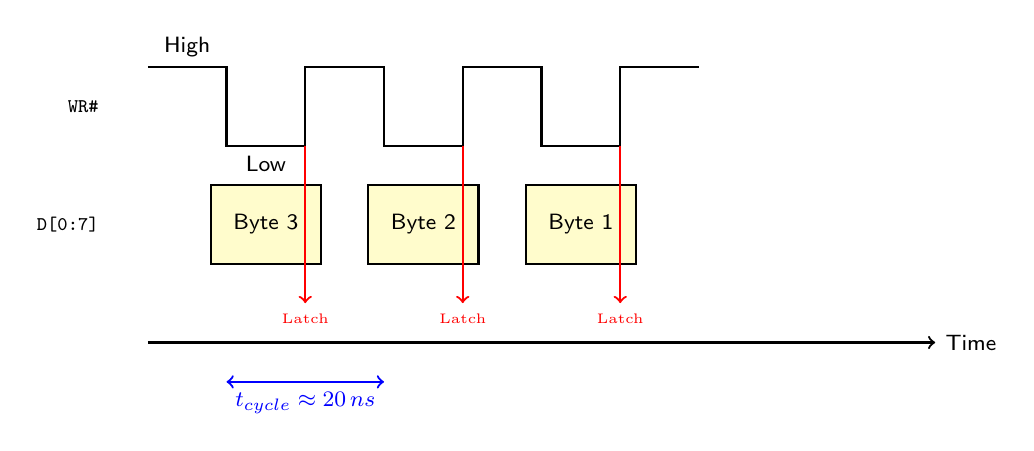
\begin{tikzpicture}[
    font=\sffamily\footnotesize,
    timing/.style={draw, thick},
    signal/.style={font=\ttfamily\scriptsize}
]

% Time axis
\draw[->,thick] (0,0) -- (10,0) node[right] {Time};

% WR# Signal
\node[signal,left] at (-0.5,3) {\texttt{WR\#}};
\draw[timing] 
    (0,3.5) -- (1,3.5) node[midway,above] {High}
    -- (1,2.5) -- (2,2.5) node[pos=0.5,below] {Low}
    -- (2,3.5) -- (3,3.5)
    -- (3,2.5) -- (4,2.5)
    -- (4,3.5) -- (5,3.5)
    -- (5,2.5) -- (6,2.5)
    -- (6,3.5) -- (7,3.5);

% Data Bus
\node[signal,left] at (-0.5,1.5) {\texttt{D[0:7]}};
\draw[timing,fill=yellow!20] 
    (0.8,1) rectangle (2.2,2) node[midway] {Byte 3};
\draw[timing,fill=yellow!20] 
    (2.8,1) rectangle (4.2,2) node[midway] {Byte 2};
\draw[timing,fill=yellow!20] 
    (4.8,1) rectangle (6.2,2) node[midway] {Byte 1};

% Latch points
\foreach \x in {2,4,6} {
    \draw[->,red,thick] (\x,2.5) -- (\x,0.5) node[below,font=\tiny] {Latch};
}

% Cycle annotation
\draw[<->,blue,thick] (1,-0.5) -- (3,-0.5) node[midway,below] {$t_{cycle} \approx 20\,\text{ns}$};

\end{tikzpicture}
}
\caption{Bus Timing Diagram. Data is stable during the low phase of \texttt{WR\#}, and the Slave latches data on the rising edge. A 20ns cycle period yields 50 MB/s throughput.}
\label{fig:bus_timing}
\end{figure}

\textbf{Key Timing Parameters}:
\begin{itemize}
    \item \textbf{$t_{cycle}$}: 20 ns (50 MHz write rate)
    \item \textbf{$t_{setup}$}: Data stable $\geq$ 5 ns before rising edge
    \item \textbf{$t_{hold}$}: Data held $\geq$ 3 ns after rising edge
\end{itemize}

\subsection{Instruction Dispatch Sequence}

Figure \ref{fig:bus_sequence} shows a complete transaction where the ESP32 (Layer 2 Master) dispatches a single \texttt{HMMA.INT8} instruction to the RP2040 (Layer 3 Slave).

\begin{figure*}[htbp]
\centering
\resizebox{0.9\textwidth}{!}{%
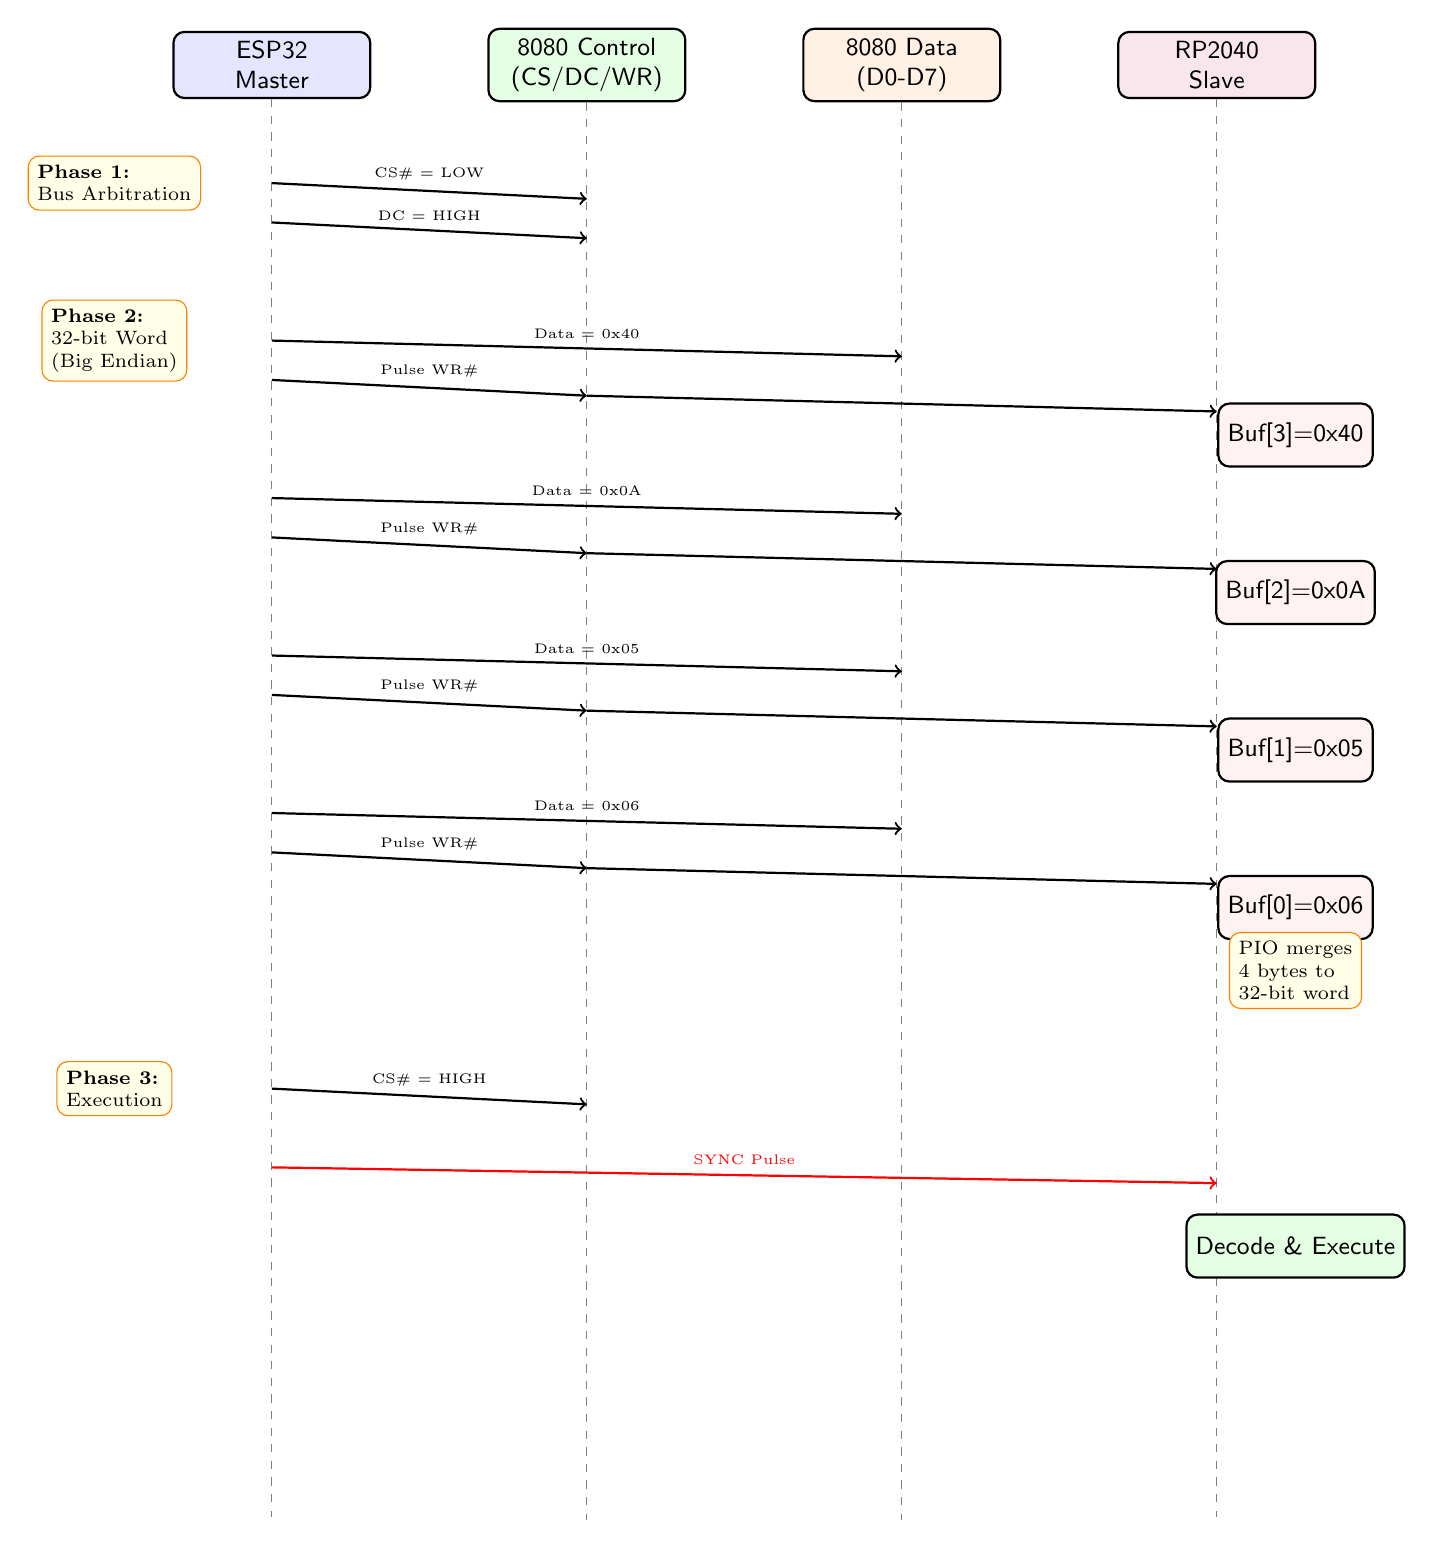
\begin{tikzpicture}[
    node distance=1.5cm,
    box/.style={rectangle, draw, thick, rounded corners, minimum width=2.5cm, minimum height=0.8cm, align=center, font=\sffamily\small},
    actor/.style={box, fill=blue!10},
    ctrl/.style={box, fill=green!10},
    data/.style={box, fill=orange!10},
    slave/.style={box, fill=purple!10},
    arrow/.style={->,thick},
    note/.style={rectangle, fill=yellow!10, draw=orange, rounded corners, align=left, font=\scriptsize}
]

% Actors
\node[actor] (master) at (0,0) {ESP32\\Master};
\node[ctrl] (bus_ctrl) at (4,0) {8080 Control\\(CS/DC/WR)};
\node[data] (bus_data) at (8,0) {8080 Data\\(D0-D7)};
\node[slave] (slave) at (12,0) {RP2040\\Slave};

% Lifelines
\foreach \n in {master,bus_ctrl,bus_data,slave} {
    \draw[dashed,gray] (\n.south) -- ++(0,-18);
}

% Phase 1: Bus Arbitration
\node[note] at (-2,-1.5) {\textbf{Phase 1:}\\Bus Arbitration};
\draw[arrow] (0,-1.5) -- node[above,font=\tiny] {CS\# = LOW} (4,-1.7);
\draw[arrow] (0,-2.0) -- node[above,font=\tiny] {DC = HIGH} (4,-2.2);

% Phase 2: Byte Transmission
\node[note] at (-2,-3.5) {\textbf{Phase 2:}\\32-bit Word\\(Big Endian)};

% Byte 3 (OpCode)
\draw[arrow] (0,-3.5) -- node[above,font=\tiny] {Data = 0x40} (8,-3.7);
\draw[arrow] (0,-4.0) -- node[above,font=\tiny] {Pulse WR\#} (4,-4.2);
\draw[arrow] (4,-4.2) -- (12,-4.4);
\node[box,fill=red!5,minimum width=1.5cm] at (13,-4.7) {Buf[3]=0x40};

% Byte 2 (Dest)
\draw[arrow] (0,-5.5) -- node[above,font=\tiny] {Data = 0x0A} (8,-5.7);
\draw[arrow] (0,-6.0) -- node[above,font=\tiny] {Pulse WR\#} (4,-6.2);
\draw[arrow] (4,-6.2) -- (12,-6.4);
\node[box,fill=red!5,minimum width=1.5cm] at (13,-6.7) {Buf[2]=0x0A};

% Byte 1 (Src1)
\draw[arrow] (0,-7.5) -- node[above,font=\tiny] {Data = 0x05} (8,-7.7);
\draw[arrow] (0,-8.0) -- node[above,font=\tiny] {Pulse WR\#} (4,-8.2);
\draw[arrow] (4,-8.2) -- (12,-8.4);
\node[box,fill=red!5,minimum width=1.5cm] at (13,-8.7) {Buf[1]=0x05};

% Byte 0 (Src2)
\draw[arrow] (0,-9.5) -- node[above,font=\tiny] {Data = 0x06} (8,-9.7);
\draw[arrow] (0,-10.0) -- node[above,font=\tiny] {Pulse WR\#} (4,-10.2);
\draw[arrow] (4,-10.2) -- (12,-10.4);
\node[box,fill=red!5,minimum width=1.5cm] at (13,-10.7) {Buf[0]=0x06};

\node[note] at (13,-11.5) {PIO merges\\4 bytes to\\32-bit word};

% Phase 3: Execution
\node[note] at (-2,-13) {\textbf{Phase 3:}\\Execution};
\draw[arrow] (0,-13) -- node[above,font=\tiny] {CS\# = HIGH} (4,-13.2);
\draw[arrow,red,thick] (0,-14) -- node[above,font=\tiny] {SYNC Pulse} (12,-14.2);
\node[box,fill=green!10] at (13,-15) {Decode \& Execute};

\end{tikzpicture}
}
\caption{Instruction Dispatch Sequence. The Master (ESP32) transmits a 32-bit HMMA instruction as four sequential bytes over the 8-bit bus. The Slave (RP2040) uses PIO to reassemble the instruction and execute upon SYNC trigger.}
\label{fig:bus_sequence}
\end{figure*}

\subsection{Hardware Implementation Notes}

\subsubsection{RP2040 Reception (PIO State Machine)}

The RP2040's Programmable I/O (PIO) is critical for achieving 50 MB/s throughput. Traditional interrupt-driven GPIO cannot sustain 20 MHz write rates. The following PIO program implements cycle-accurate bus reception:

\begin{lstlisting}[caption={RP2040 PIO Program for 8080 Bus Reception},label={lst:pio_rx}]
.program parallel_8080_rx
.wrap_target
    wait 0 pin 10      ; Wait for CS# low (Pin 10)
    wait 0 pin 11      ; Wait for WR# low (Pin 11)
    
    in pins, 8         ; Read 8-bit D0-D7 into ISR
    
    wait 1 pin 11      ; Wait for WR# rising edge
.wrap

; Configuration:
; - Auto-push enabled when ISR full (32 bits = 4 bytes)
; - CPU reads complete 32-bit instruction from RX FIFO
\end{lstlisting}

This PIO program runs autonomously, allowing the CPU to process instructions only when a complete 32-bit word is available in the FIFO.

\subsubsection{Signal Integrity Considerations}

To ensure reliable operation at 50 MB/s:

\begin{itemize}
    \item \textbf{Trace Length Matching}: All 8 data lines (\texttt{D[0:7]}) should be routed with $\pm$1 mm length tolerance to prevent skew.
    \item \textbf{GPIO Drive Strength}: Configure AMB82 and ESP32 GPIO pads for high drive current (20 mA recommended) to support multiple parallel loads.
    \item \textbf{Termination}: For cables longer than 10 cm, consider 100$\Omega$ series termination resistors on \texttt{WR\#} and \texttt{CS\#} to reduce reflections.
    \item \textbf{Ground Planes}: Use a continuous ground plane under the bus traces to minimize crosstalk and EMI.
\end{itemize}

\subsection{Performance Analysis}

The theoretical maximum throughput is determined by the \texttt{WR\#} toggle rate:

\[
\text{Bandwidth} = \frac{8 \text{ bits}}{t_{cycle}} = \frac{8 \text{ bits}}{20 \text{ ns}} = 400 \text{ Mbps} = 50 \text{ MB/s}
\]

In practice, overhead from \texttt{CS\#} assertion, DMA setup, and FIFO latency reduces effective throughput to approximately 40-45 MB/s for sustained transfers. This is sufficient for streaming weights and instructions in real-time neural network inference workloads.
